\chapter{Introduction}\label{introchapter}
The auditory system is among the most ubiquitious of sensory systems as evidenced by the 
development of numerous strategies for the detection and processing of auditory stimuli
across several species. The processing of sound stimuli is fairly fast and in comparison
to light stimuli, sound has two main properties - it is omnidirectional and due to
its large wavelength, it isn't blocked by small objects. For instance we can hear objects
behind us or behind obstacles whereas the same isn't true for visual stimuli. These properties 
give the animal the obvious advantage of being able to react to approaching dangers that
aren't yet visible. In order to fully utilize the sound stimuli, it is therefore essential
that an animal is able to assess the direction or \textit{localize} a sound source.


\begin{figure}
 %\centering
 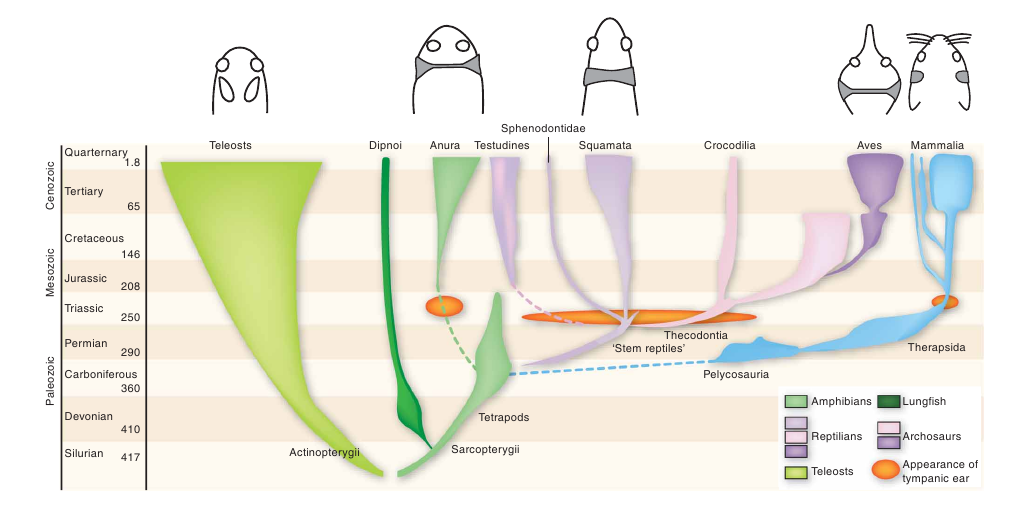
\includegraphics[width=1.0\linewidth]{Diagrams/vertebrateearevolution.png}
 \caption[Vertebrate Ear Evolution]{Figure due to Schnupp and Carr \cite{schnuppcarr}.}
 \label{vertebrateearevolution}
\end{figure}